\documentclass{beamer}
\usetheme{metropolis}

\usepackage[spanish,es-noshorthands]{babel}
\usepackage[utf8]{inputenc}
\usepackage{graphicx}
\usepackage{tikz}
\usepackage{xcolor}
\usepackage{amsmath}
\usepackage{listings}
\usepackage{upquote}
\usepackage[T1]{fontenc}
\usepackage{lmodern}
\usepackage{cmap}
\usepackage{inconsolata}
\usepackage{listingsutf8}
\input{glyphtounicode}
\pdfgentounicode=1

\lstset{
    language=Python,
    basicstyle=\tiny\ttfamily,
    numbers=none,
    breaklines=false,
    keepspaces=true,
    showstringspaces=false,
    upquote=true,
    tabsize=4,
    columns=fullflexible,
    inputencoding=utf8
}

\usetikzlibrary{positioning,shapes.multipart,calc,arrows,shapes.geometric}

% Definición de colores personalizados
\definecolor{primary}{RGB}{46, 204, 113}
\definecolor{secondary}{RGB}{52, 152, 219}
\definecolor{accent}{RGB}{231, 76, 60}
\definecolor{background}{RGB}{236, 240, 241}
\definecolor{gradient1}{RGB}{255, 107, 107}
\definecolor{gradient2}{RGB}{255, 159, 67}

% Configuración del tema
\setbeamercolor{normal text}{fg=black,bg=background}
\setbeamercolor{structure}{fg=primary}
\setbeamercolor{alerted text}{fg=accent}

\title{\Huge\textbf{Instalación de Software para I.O.}}
\author{Investigación Operativa}
\date{}

\begin{document}

\begin{frame}
    \titlepage
    \begin{tikzpicture}[remember picture,overlay]
        \node[anchor=south west,inner sep=30pt] at (current page.south west) {
            
\includegraphics[height=1cm]{../misc/UdeSA.png}
        };
    \end{tikzpicture}
\end{frame}

\begin{frame}{Cosas que vamos a instalar}
    \begin{itemize}
        \item \textbf{Anaconda}: para instalar y gestionar entornos de Python de forma sencilla.
        \item \textbf{Spyder}: el entorno de desarrollo que vamos a usar para correr archivos de Python con librerías específicas de investigación operativa.
    \end{itemize}
    Primero instalamos Anaconda, que nos permite crear entornos y después instalamos Spyder dentro del entorno para asegurarnos de que tenga todas las librerías necesarias.
\end{frame}

\begin{frame}{Espacio necesario en disco}
    \begin{center}
        {\LARGE Antes de instalar Anaconda y Spyder, asegurate de tener al menos 5GB de espacio libre en tu disco.}
    \end{center}
\end{frame}

\begin{frame}{Web de Anaconda Navigator}
    Para descargar Anaconda Navigator, anda a la web oficial y tocá el botón para descargarlo.

    \vspace{0.3cm}
    \href{https://www.anaconda.com/download/success}{\textcolor{secondary}{\textbf{https://www.anaconda.com/download/success}}}
    
    \vspace{0.5cm}
    \centering
    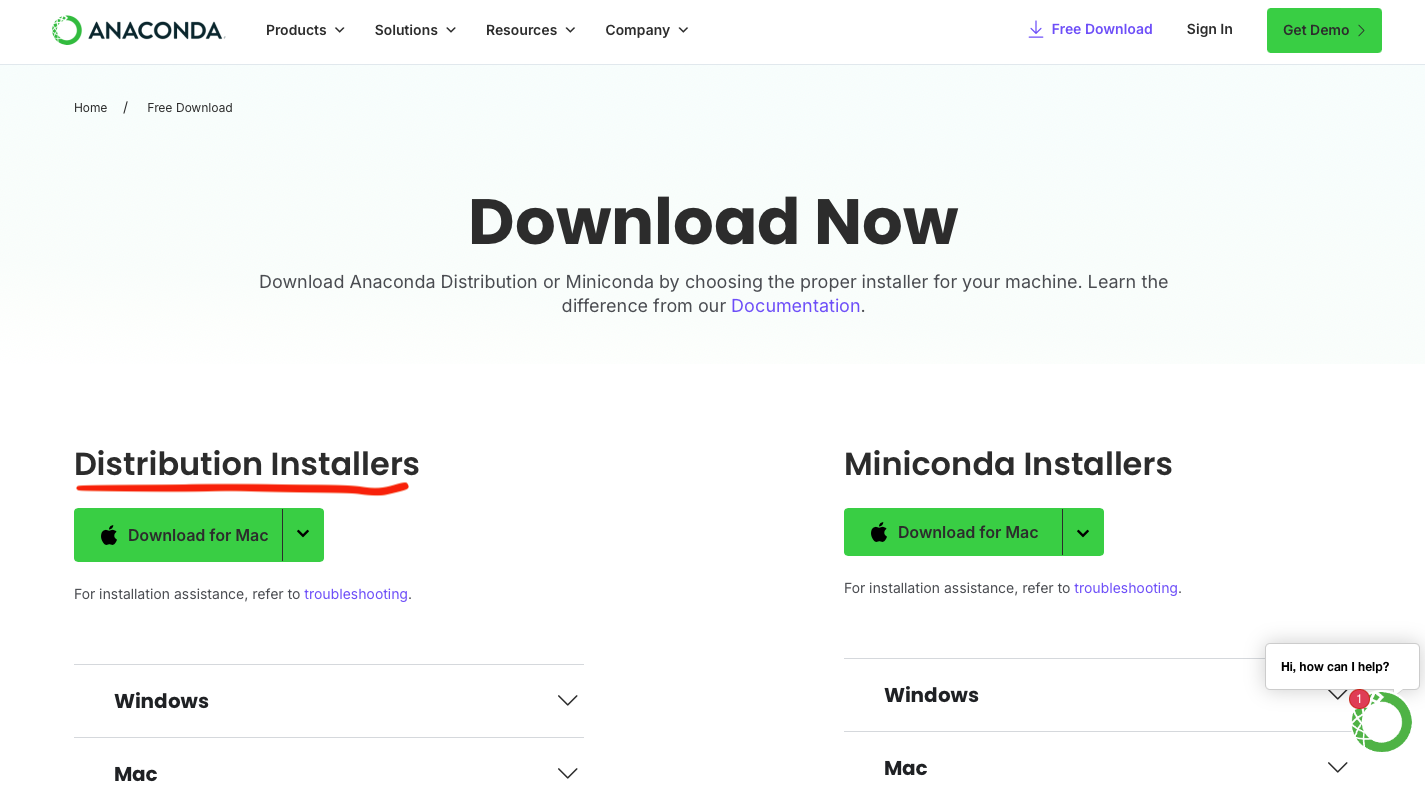
\includegraphics[width=0.6\textwidth]{img/anaconda_download.png}
\end{frame}

\begin{frame}{Descargando}
    \begin{center}
        Si tenés Mac, tenés que fijarte si tenes una con un procesador Intel o si tenés una con procesador tipo M1, M2, etc. Si tenes uno de esos M1/M2/etc entonces seleccioná la opción de Apple Silicon. Si tenes Windows seleccionás la de Windows.
        
        \vspace{0.5cm}
        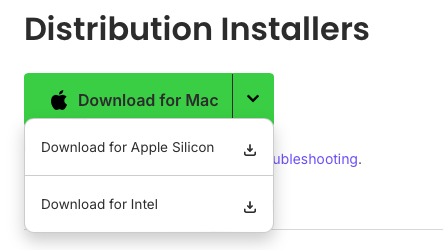
\includegraphics[width=0.6\textwidth]{img/anaconda_mac.png}
    \end{center}
\end{frame}

\begin{frame}{Instalar}
    \begin{center}
        En Mac vas a abrir el .pkg que se te bajó y tocar todo continuar para instalarlo. En Windows es lo mismo.
        
        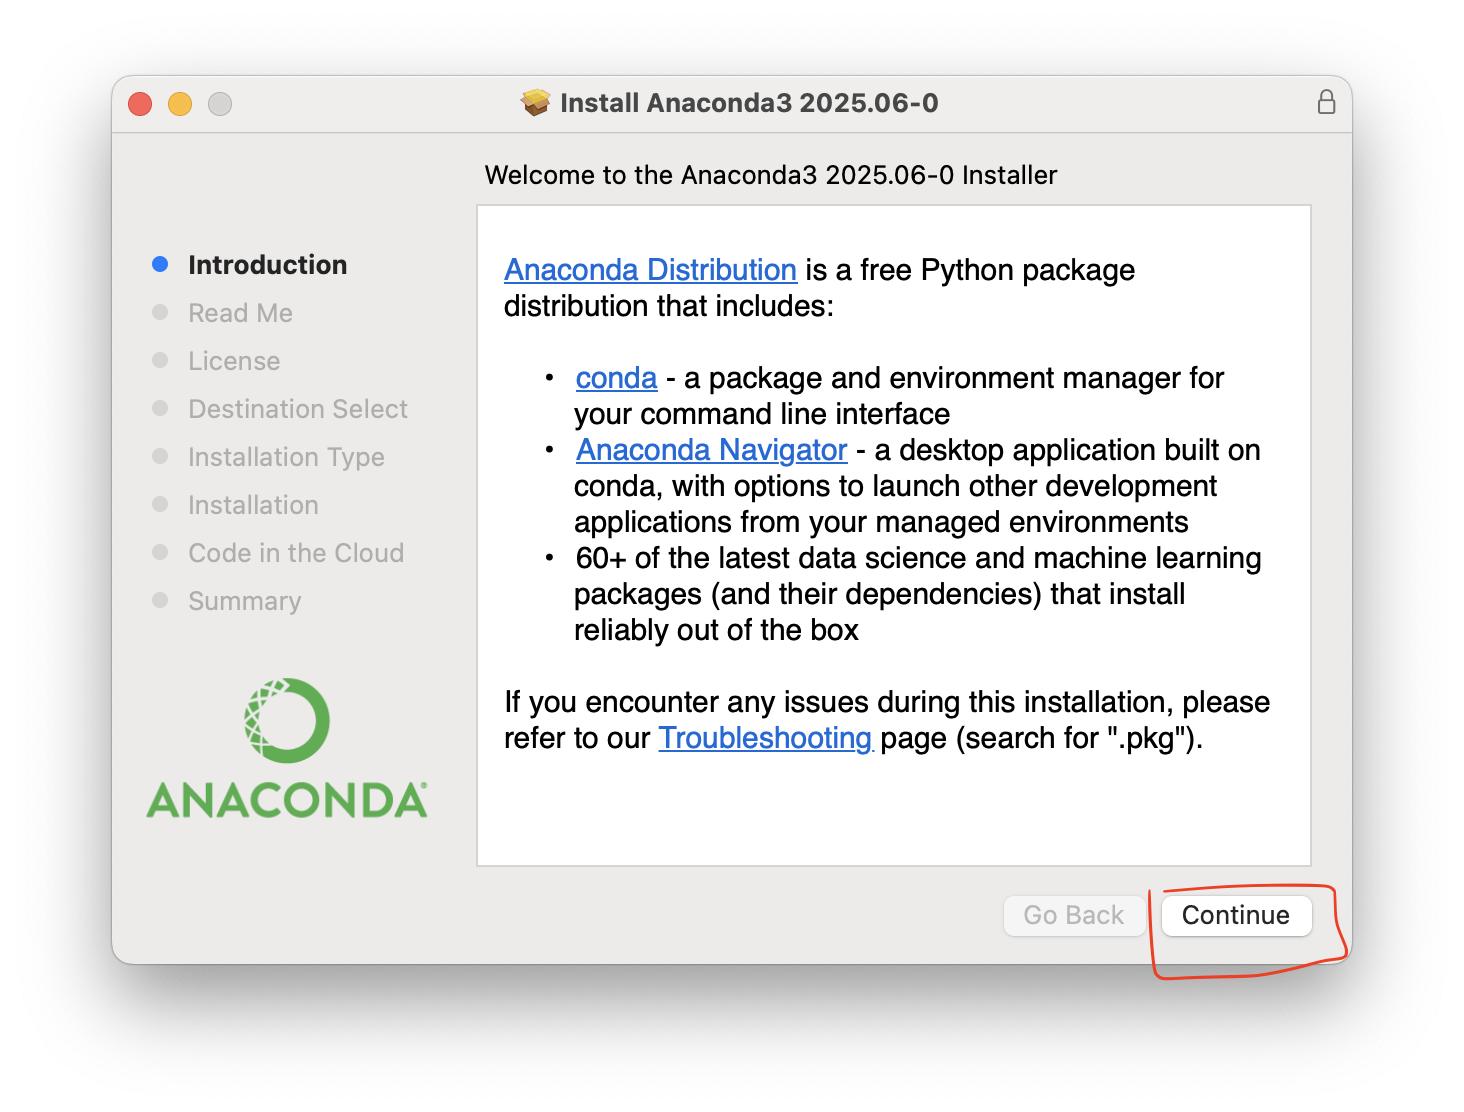
\includegraphics[width=0.9\textwidth]{img/todo_continuar_perro.png}
    \end{center}
\end{frame}

\begin{frame}{Podría pasar este error y entonces haces esto}
    \begin{center}
        \textcolor{red}{\textbf{¡¡Solo si tenes Mac!!}}
    \end{center}
    Si te tira que no podés instalarlo porque ya hay algo en /opt/anaconda3 entonces abris la terminal y tirás el siguiente comando. No vas a ver tu contraseña cuando la escribas. Después probas instalar de vuelta.

    \begin{center}
        \begin{minipage}{0.48\textwidth}
            \centering
            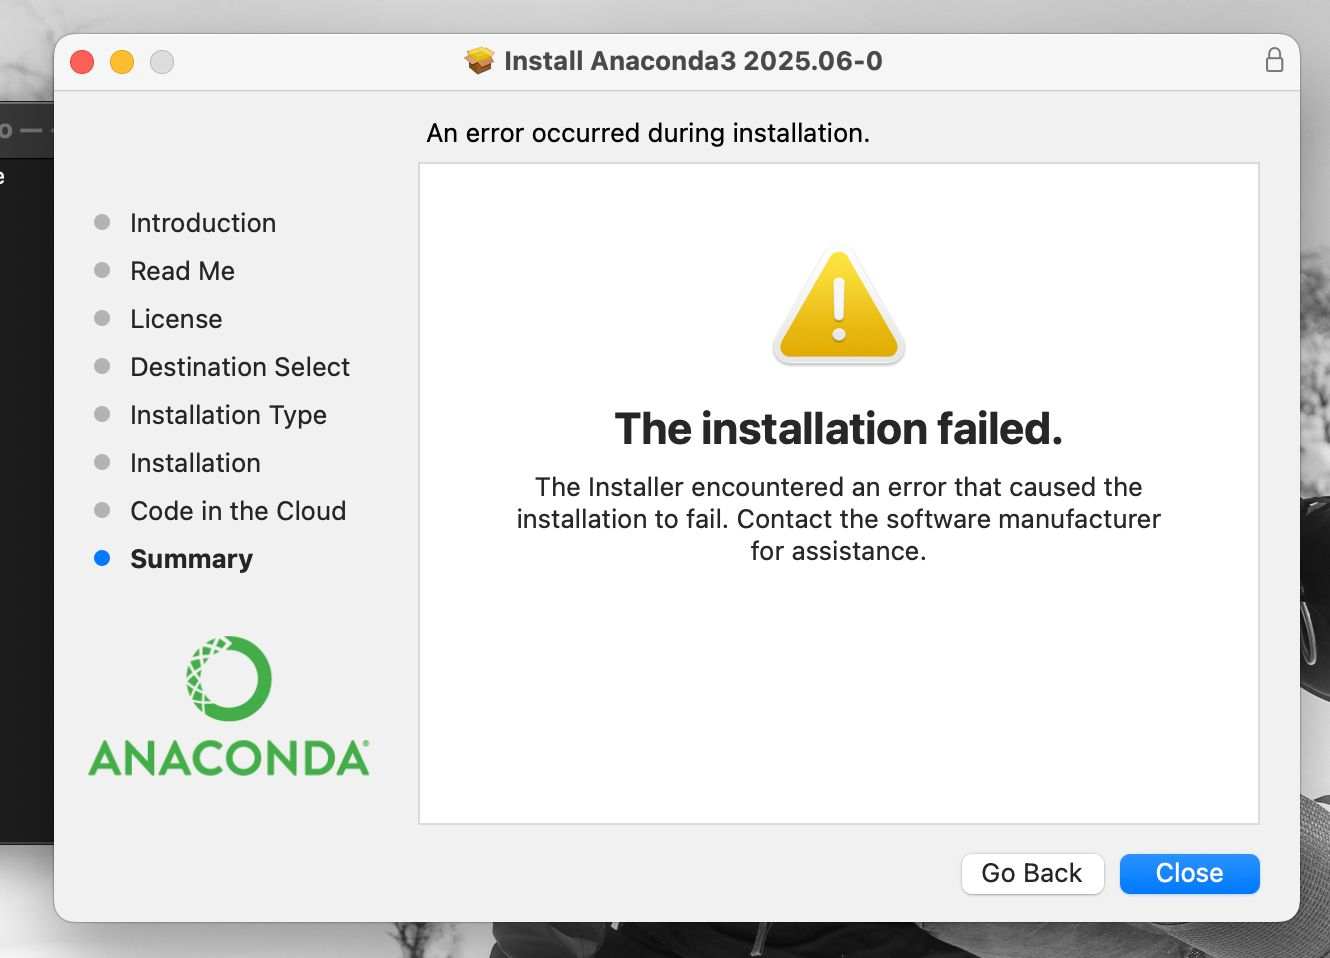
\includegraphics[width=\textwidth]{img/error_mac_opt.jpeg}
        \end{minipage}
        \hfill
        \begin{minipage}{0.48\textwidth}
            \centering
            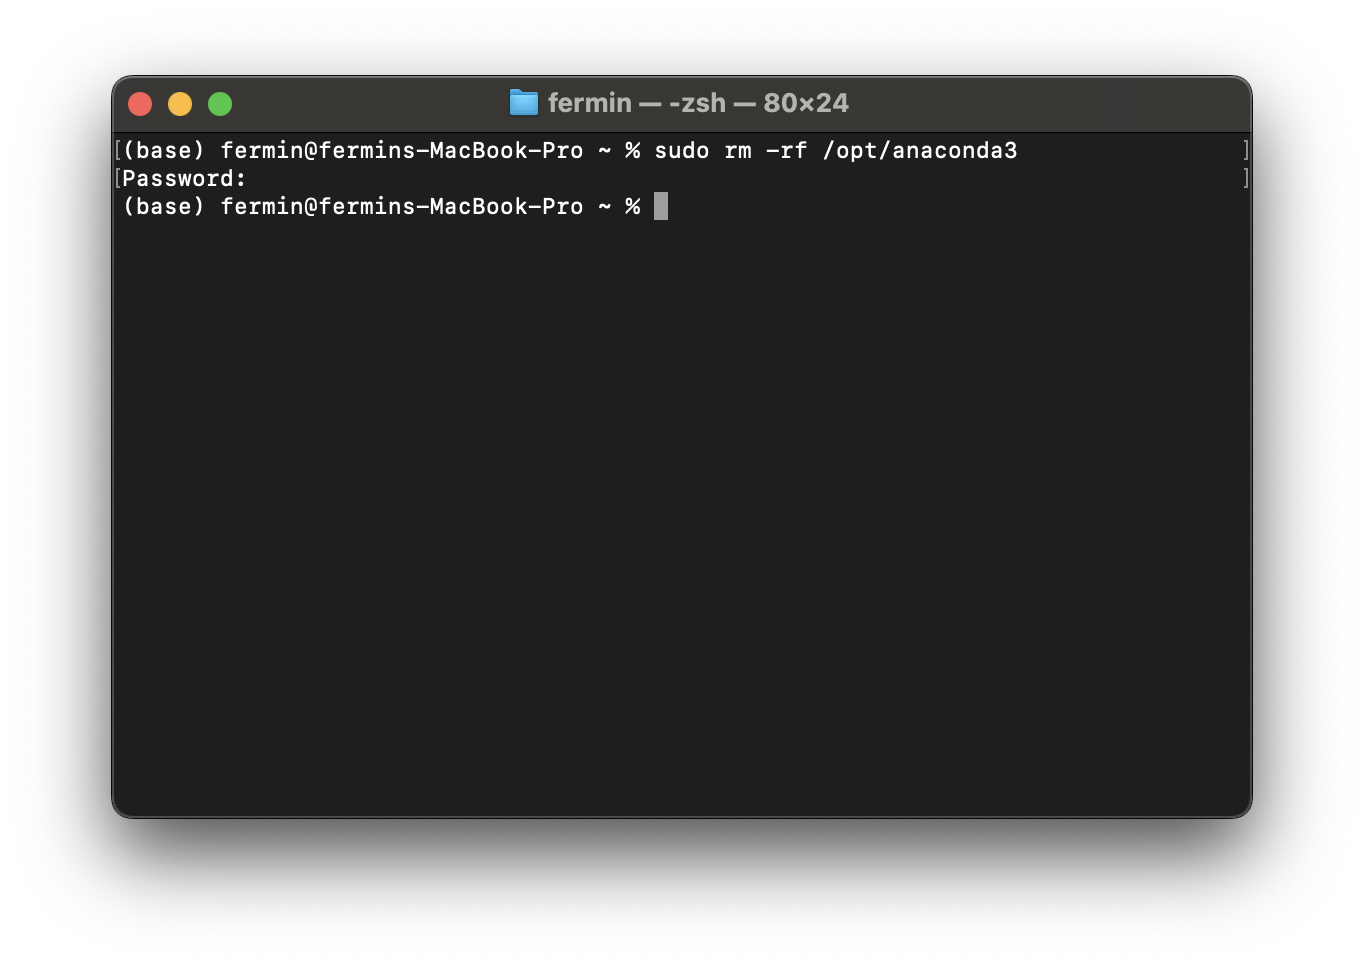
\includegraphics[width=\textwidth]{img/comando_sudormrf.png}
        \end{minipage}
    \end{center}
\end{frame}

\begin{frame}{Podría pasar este error y entonces haces esto}
    \begin{center}
        \textcolor{red}{\textbf{¡¡Solo si tenes Windows!!}}
    \end{center}
    Si te tira que no podés instalarlo porque ya hay algo en la carpeta entonces abris el explorador de archivos y vas a ir a borrar esa carpeta. Después probas instalar de vuelta.

    \begin{center}
        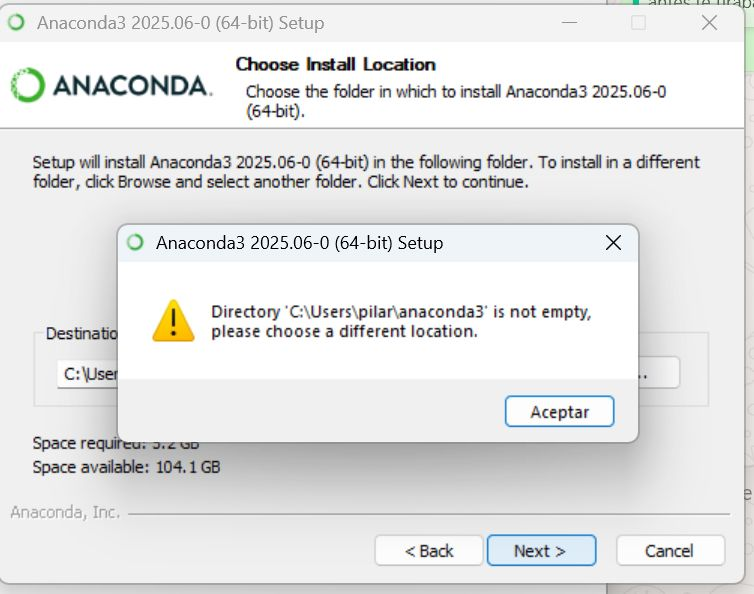
\includegraphics[width=0.6\textwidth]{img/windows_folder_not_empty.jpeg}
    \end{center}
\end{frame}

\begin{frame}{Abrís Anaconda Navigator}
    Si todo salió bien y pudiste abrir Anaconda Navigator se debería ver así y vamos a ir a Environments.
    \begin{center}
        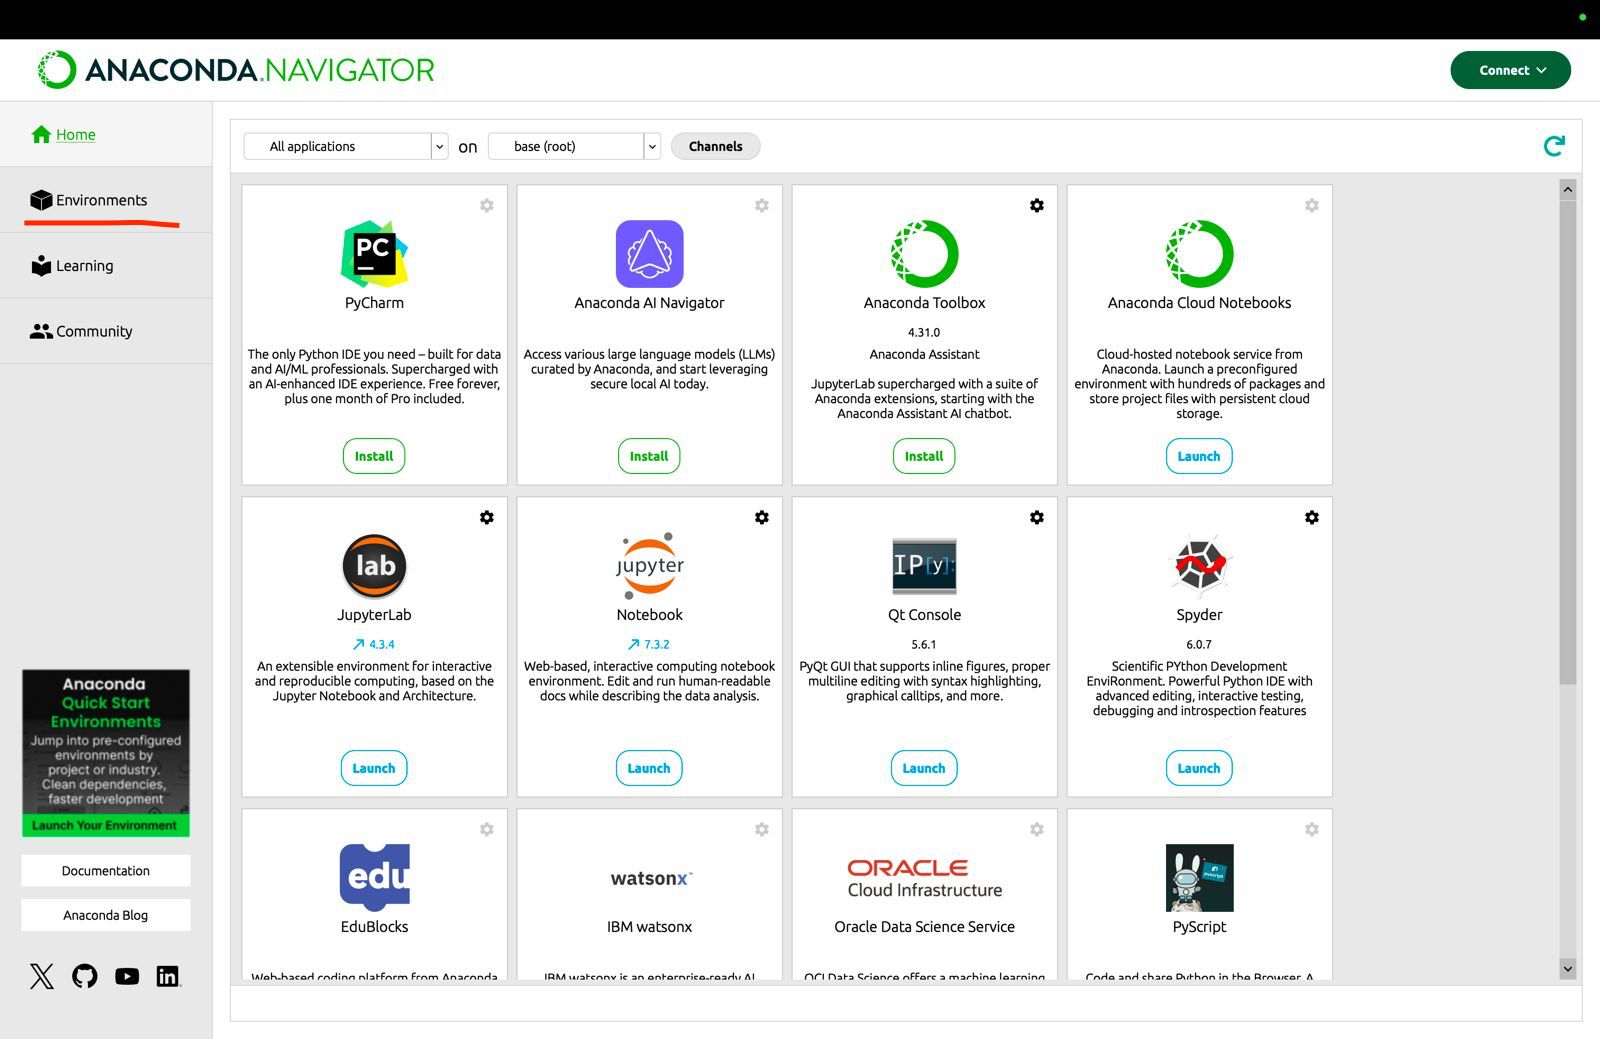
\includegraphics[width=0.8\textwidth]{img/anaconda_navigator.jpeg}
    \end{center}
\end{frame}

\begin{frame}{Importamos el ambiente}
    Hacemos click en el de ``Importar'' para poder subir el .yml que bajamos del repo de github.
    \begin{center}
        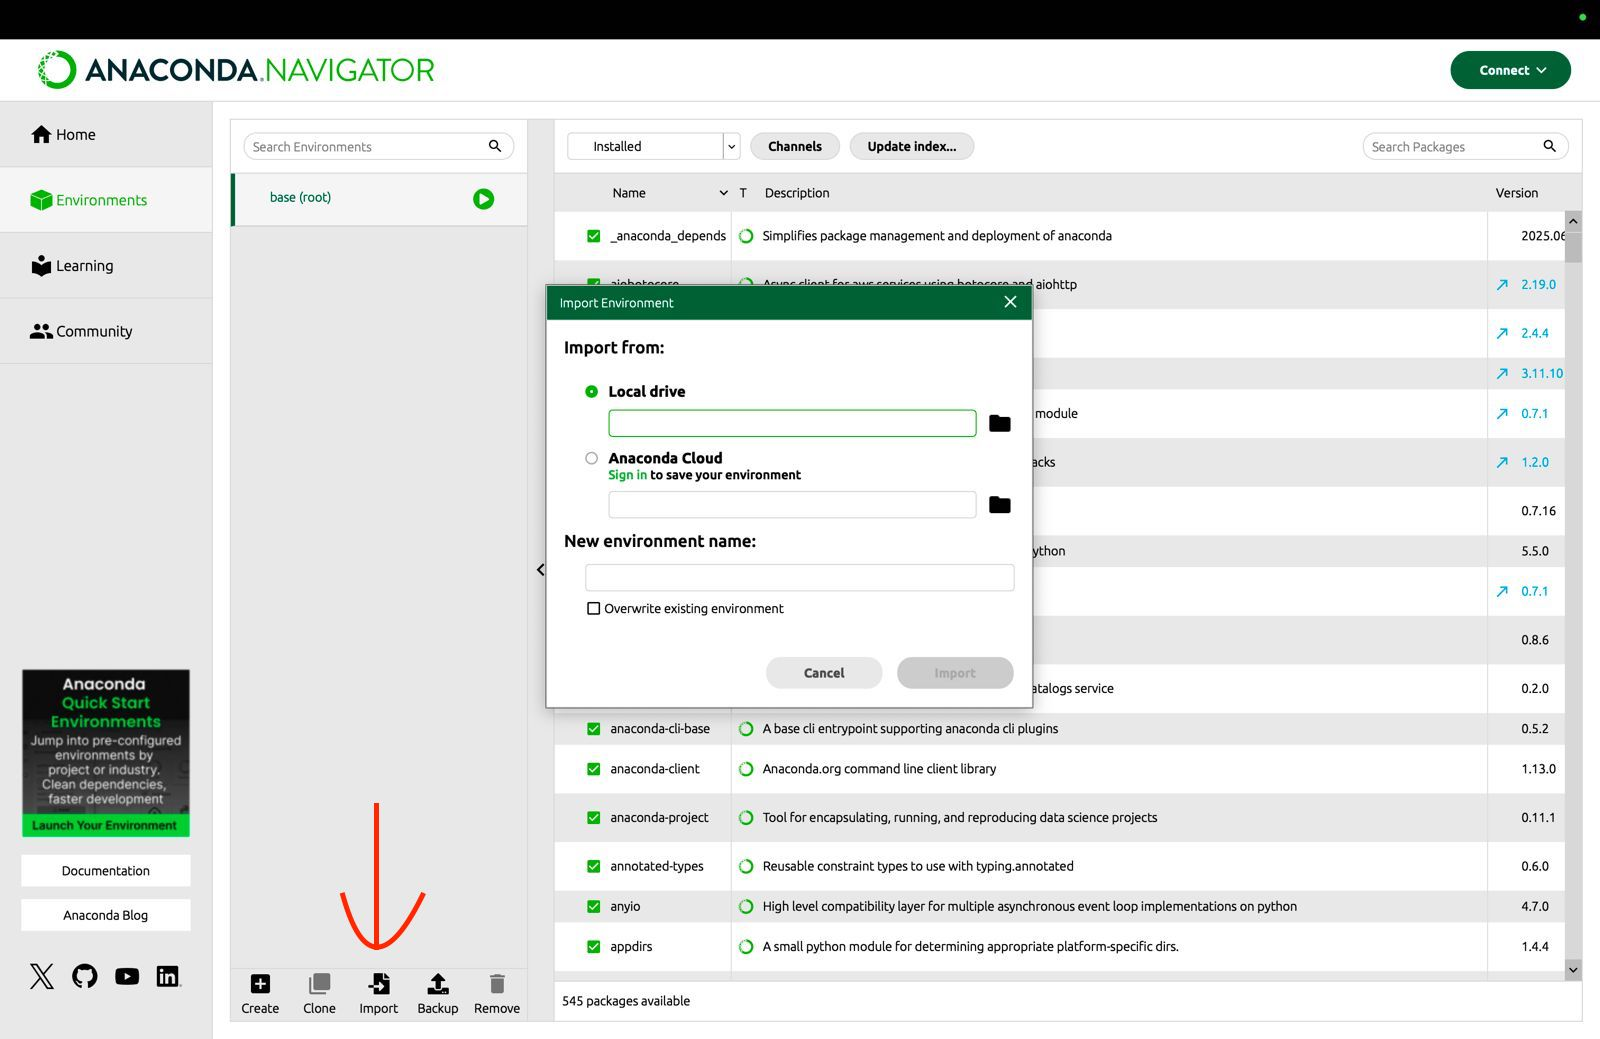
\includegraphics[width=0.8\textwidth]{img/import_environment.jpeg}
    \end{center}
\end{frame}

\begin{frame}{Buscamos el .yml}
    Van a buscar el .yml que está en la carpeta de esta clase en el repo de github y bajarlo.
    \begin{center}
        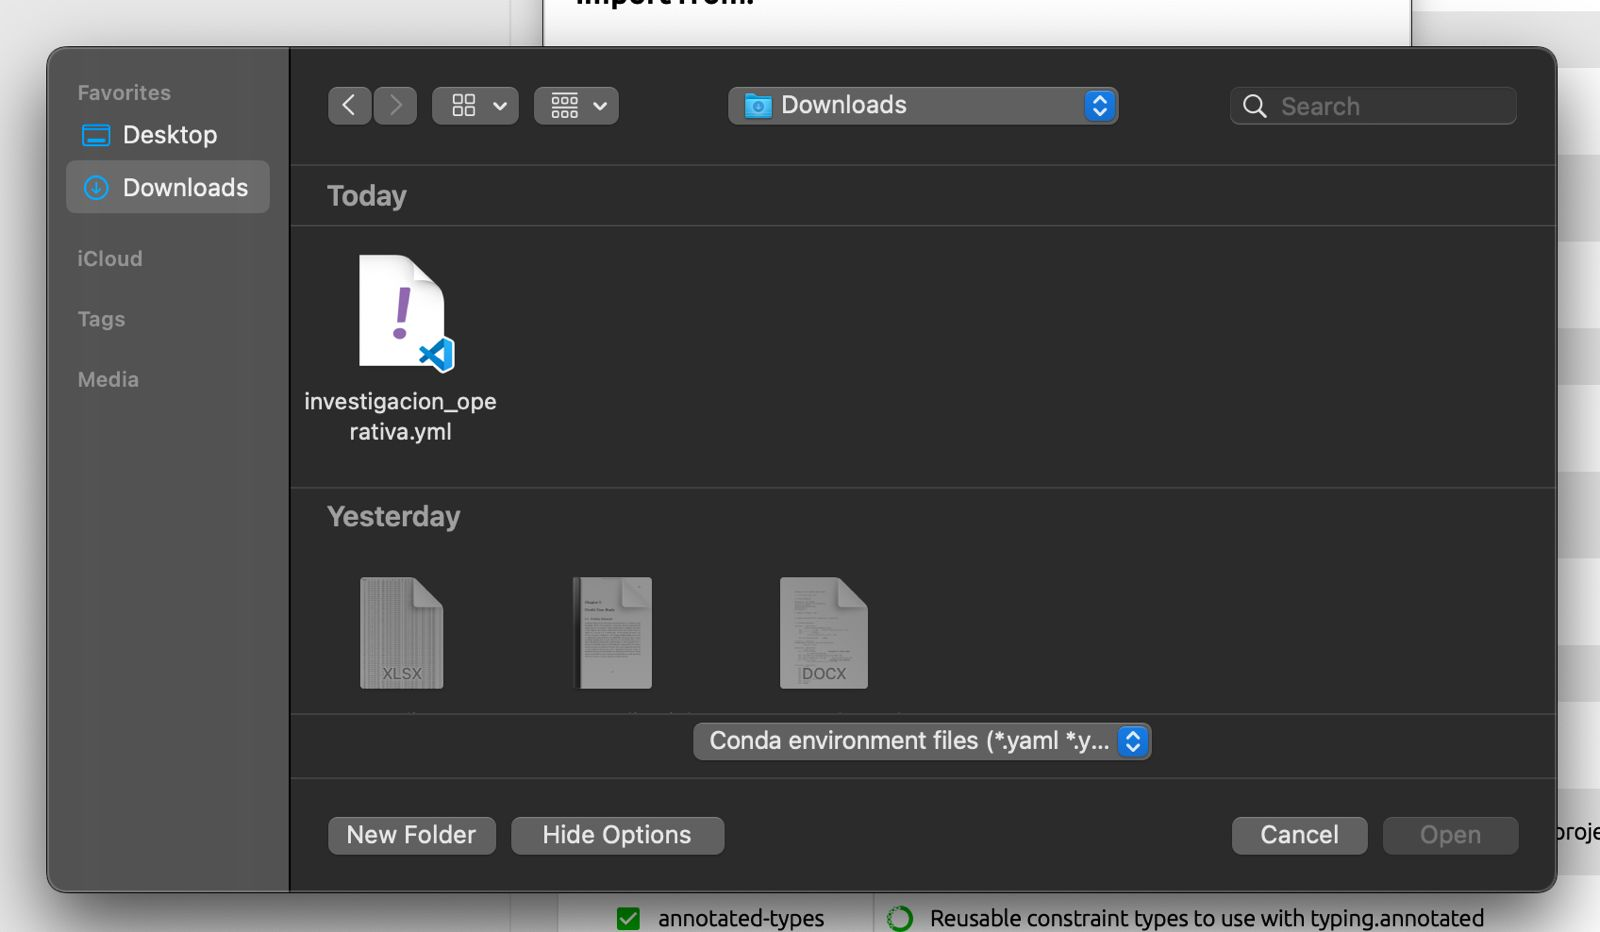
\includegraphics[width=0.8\textwidth]{img/yml.jpeg}
    \end{center}
\end{frame}

\begin{frame}{Ambiente creado}
    Fijensé de que esté en verde con el play ahí en el ambiente que acabamos de hacer y no otro.
    \begin{center}
        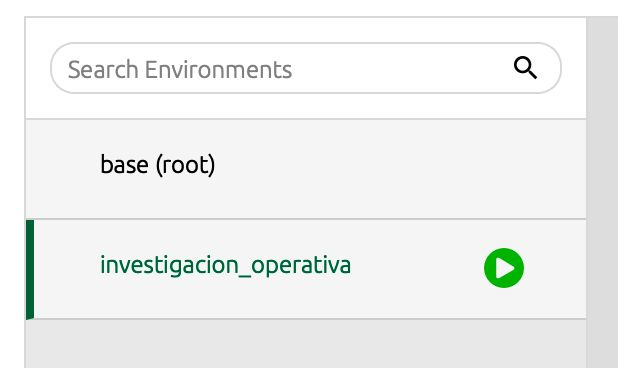
\includegraphics[width=0.8\textwidth]{img/ambiente_creado.jpeg}
    \end{center}
\end{frame}

\begin{frame}{Abrimos Spyder}
    \begin{center}
        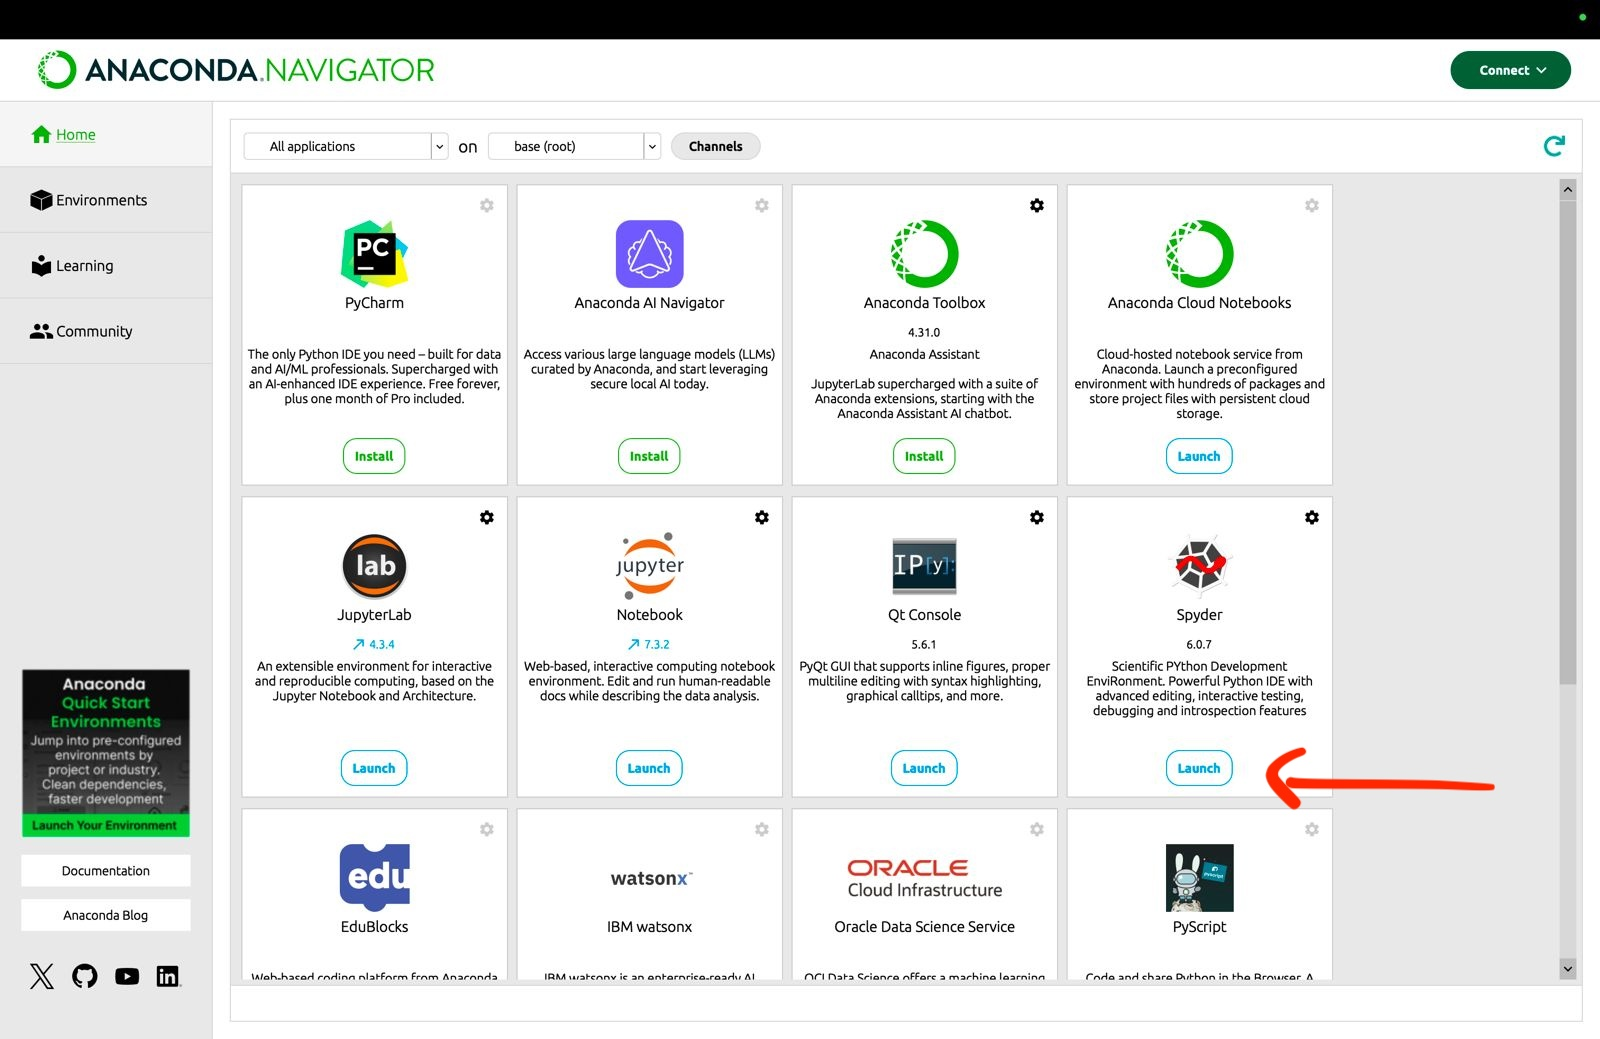
\includegraphics[width=0.8\textwidth]{img/spyder.jpeg}
    \end{center}
\end{frame}

\begin{frame}[fragile]{Ejemplo de uso de picos}
\begin{columns}
\begin{column}{0.45\textwidth}
Vamos a copiar el código de la derecha y pegarlo en el editor de Spyder. Después tocamos play y vemos si a la derecha abajo vemos un resultado. Si es así, entonces tenemos la instalación de Spyder completa.
\end{column}
\begin{column}{0.55\textwidth}
\begin{lstlisting}
import picos
import numpy as np

P = picos.Problem()

x = picos.RealVariable('x', 2)

A = np.array([
    [2, 3],
    [3, 2]
])
b = np.array([100, 80])
c = np.array([40, 30])

A = picos.Constant('A', A)
b = picos.Constant('b', b)
c = picos.Constant('c', c)

P.set_objective('max', c | x)
P.add_constraint(A * x <= b)
P.add_constraint(x >= 0)

P.solve(solver='glpk')
print(f"x1 = {x[0].value:.2f}, x2 = {x[1].value:.2f}")
print(f"Z = {P.value:.2f}")
\end{lstlisting}
\end{column}
\end{columns}
\end{frame}

\begin{frame}{Éxito}
    Si vemos la solución en la consola significa que tenemos todo instalado y podemos hacer las guías en nuestra computadora.
    \begin{center}
        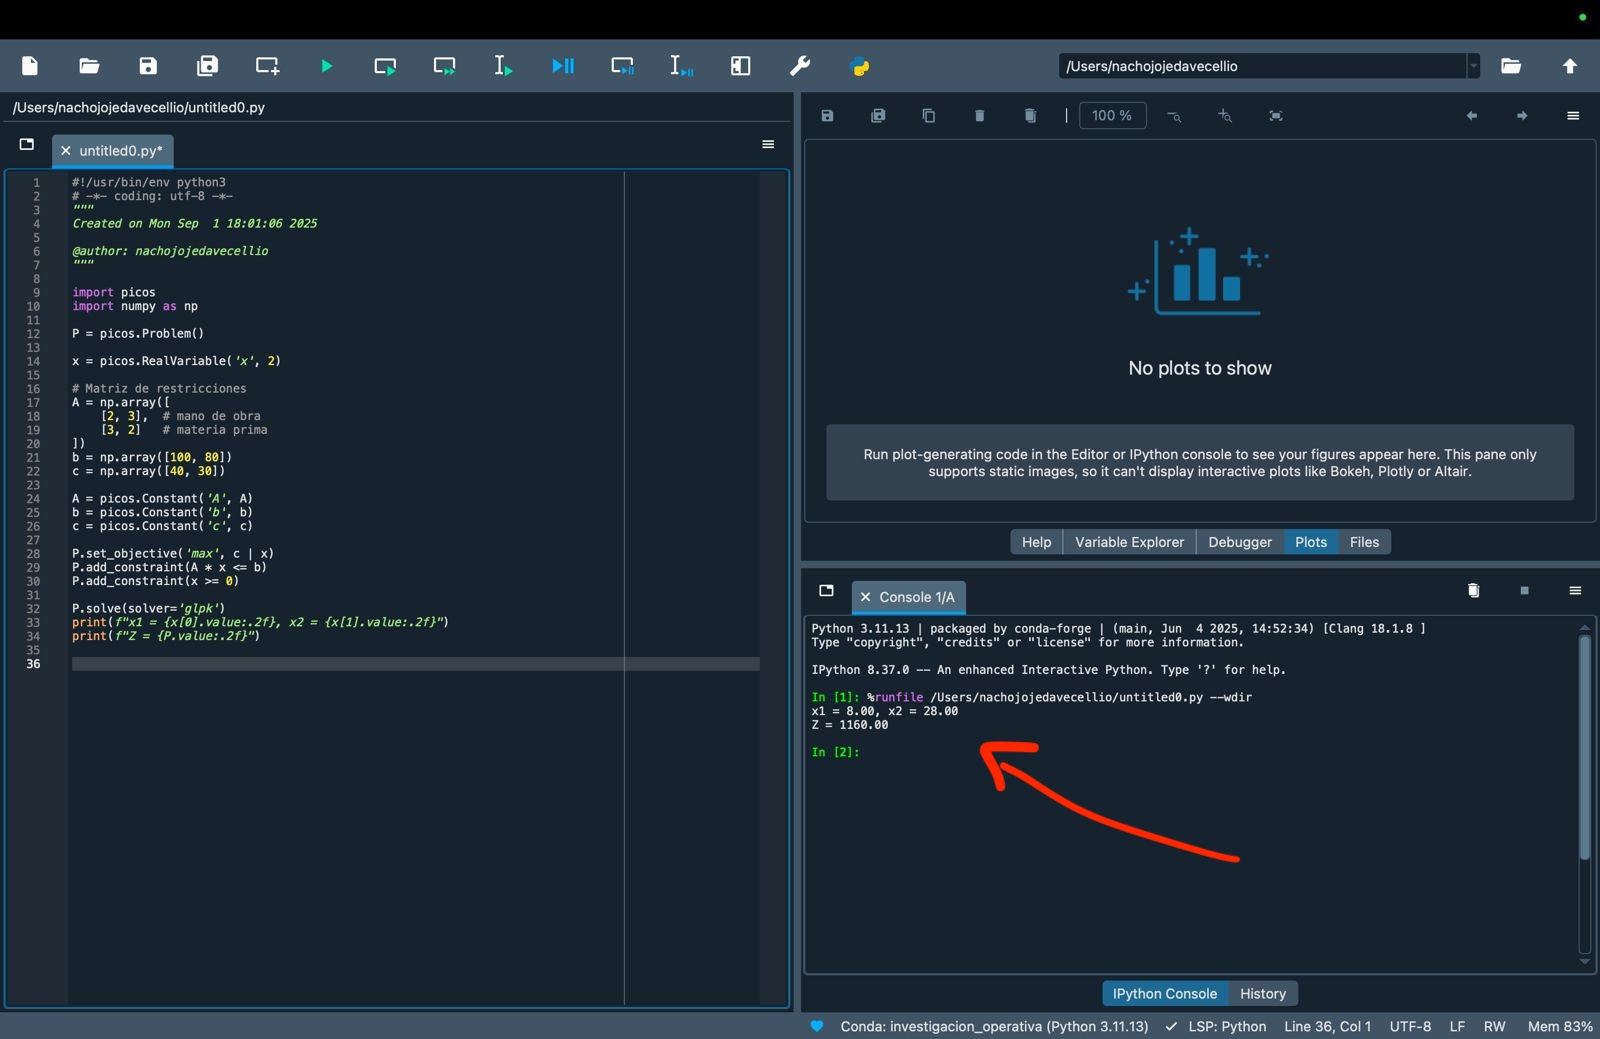
\includegraphics[width=0.8\textwidth]{img/exito.jpeg}
    \end{center}
\end{frame}

\end{document}
